\documentclass[10pt]{article}
\usepackage{amsmath,amssymb}
\usepackage{ctex}
\usepackage{multicol}
\usepackage{geometry}
\usepackage{array}
\usepackage{float}
\usepackage{tikz}
\usetikzlibrary{automata}
\usepackage[ruled]{algorithm2e}
\geometry{left=1cm,right=1cm,top=1cm,bottom=1.5cm}
\title{编译原理混子速成}
\date{}
\begin{document}
	\begin{multicols}{3}
		\maketitle
		\paragraph{闭包}
		\begin{align*}
			A^0 &=\{\epsilon\} \\
			A^+ &= \cup_{i=1}^\infty A^i\\
			A^* &= \cup_{i=0}^\infty A^i
		\end{align*}
		\paragraph{文法} $ G[S]=(V_N, V_T, P, S) $
		\paragraph{正则表达式代数定律}\hfill
		
			\noindent\begin{tabular}{|c|c|}
				\hline
				定律 & 描述 \\
				\hline
				$r|s=s|r$ & $|$是可以交换的 \\
				\hline
				$r|(s|t)=(r|s)|t$ & $|$是可结合的 \\
				\hline
				$r(st)=(rs)t$ & 连接是可结合的 \\
				\hline
				$r(s|t)=rs|rt$ & 连接对$|$是可分配的 \\
				$(s|t)r=sr|tr$ & \\
				\hline
				$\epsilon r = r\epsilon = r$& $\epsilon$是连接的单位元 \\
				\hline
				$r^*=(r|\epsilon)^*$& 闭包一定包含$\epsilon$ \\
				\hline
				$r^{**}=r^*$ & $*$具有等幂性 \\
				\hline
			\end{tabular}
		
		\paragraph{NFA 状态集上的操作}\hfill
		
		\noindent\begin{tabular}{|c|p{9em}|}
			\hline
			操作 & 描述 \\
			\hline
			$ \epsilon-closure(s) $ & 能够从NFA的状态$ s $开始只通过$\epsilon$转换到达的NFA状态的集合 \\
			\hline
			$ \epsilon-closure(T) $& 能够从$ T $中的某个NFA状态$ s $开始只通过$\epsilon$转换到达的NFA状态集合 \\
			\hline
			$ move(T,a) $& 能够从$ T $中的某个状态$ s $出发通过标号为$ a $的转换到达的NFA状态的集合 \\
			\hline
		\end{tabular}
		
		\begin{algorithm}[H]
			\caption{子集构造法}
			$\epsilon-closure(s_0)$是\textit{Dstates}中的唯一状态,且未加标记\;
			\While{在\textit{Dstates}中有一个未标记状态$T$}{
				给$ T $加上标记\;
				\For{每个输入符号 $ a $}{
					$U=\epsilon-closure(move(T,a))$\;
					\If{$U$不在\textit{Dstates}中}{
						将 $U$ 加入到 \textit{Dstates} 中,且不加标记\;
					}
					$Dtran[T,a]=U$\;
				}
			}
		\end{algorithm}
		
		\paragraph{构造NFA}\hfill
		
		\noindent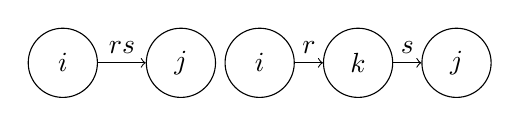
\begin{tikzpicture}
			\node[state] (v1) at (-2,1.5) {$i$};
			\node[state] (v2) at (-0.5,1.5) {$j$};
			\draw[->] (v1) edge node[above] {$rs$} (v2);
			\node[state] (v3) at (0.5,1.5) {$i$};
			\node[state] (v4) at (1.75,1.5) {$k$};
			\node[state] (v5) at (3,1.5) {$j$};
			\draw[->] (v3) edge node[above] {$r$} (v4)
				(v4) edge node [above] {$s$} (v5); 
		\end{tikzpicture}
		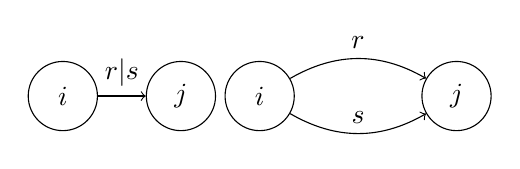
\begin{tikzpicture}
			\node[state] (v1) at (-2,1.5) {$i$};
			\node[state] (v2) at (-0.5,1.5) {$j$};
			\draw[->] (v1) edge node[above] {$r|s$} (v2);
			\node[state] (v3) at (0.5,1.5) {$i$};
			\node[state] (v5) at (3,1.5) {$j$};
			\draw[->] (v3) edge[bend left] node[above] {$r$} (v5)
			(v3) edge[bend right] node [above] {$s$} (v5); 
		\end{tikzpicture}
		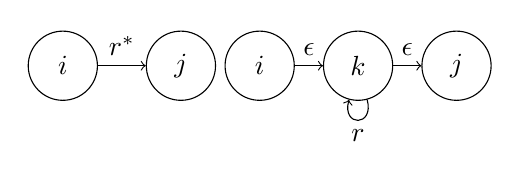
\begin{tikzpicture}
			\node[state] (v1) at (-2,1.5) {$i$};
			\node[state] (v2) at (-0.5,1.5) {$j$};
			\draw[->] (v1) edge node[above] {$r^*$} (v2);
			\node[state] (v3) at (0.5,1.5) {$i$};
			\node[state] (v4) at (1.75,1.5) {$k$};
			\node[state] (v5) at (3,1.5) {$j$};
			\draw[->] (v3) edge node[above] {$\epsilon$} (v4)
			(v4) edge node [above] {$\epsilon$} (v5);
			\draw[->] (v4) edge[loop below, looseness=4] node  {$r$} (v4); 
		\end{tikzpicture}
	
		\paragraph{消除左递归}
		\begin{equation*}
			A \rightarrow A\alpha | \beta \Rightarrow \begin{cases}
				A\rightarrow \beta A^\prime\\
				A^\prime \rightarrow \alpha A^\prime | \epsilon
			\end{cases}
		\end{equation*}
		\begin{algorithm}[H]
			\caption{消除左递归}
			按照某个顺序将非终结符号排序为 $A_1,A_2,\cdots,A_n$\;
			\For{$i\leftarrow 1$ to $n$}{
				\For{$j\leftarrow 1$ to $i-1$}{
					$A_i\rightarrow A_j \gamma, A_j\rightarrow \delta_1|\delta_2|\cdots|\delta_n\Rightarrow A_i \rightarrow \delta_1\gamma|\delta_2\gamma|\cdots|\delta_k\gamma$\;	
			}
			消除$A_i$产生式之间的立即左递归\;
			}
		\end{algorithm}
		\paragraph{提取左公因子}
		\begin{equation*}
			A\rightarrow \alpha\beta_1|\alpha\beta_2 \Rightarrow \begin{cases}
				A\rightarrow \alpha A^\prime \\
				A^\prime \rightarrow \beta_1 |\beta_2
			\end{cases}
		\end{equation*}
		\paragraph{FIRST}
		\begin{itemize}
			\item $X$ 是终结符号,FIRST($X$) = $X$。
			\item $X$ 是非终结符号,
			\begin{equation*}
				\begin{cases}
					X\rightarrow a\alpha,\text{则 }a\in\text{FIRST}(X)\\
					X\rightarrow \epsilon,\text{则 }\epsilon \in\text{FIRST}(X)
				\end{cases}
			\end{equation*}
			\item $X\rightarrow Y_1Y_2\cdots Y_k$
			\begin{enumerate}
				\item $Y_1$ 是非终结符,FIRST$(Y_1)-\{\epsilon\}\subseteq$FIRST($X$)。
				\item $Y_1Y_2\cdots Y_i(1\leq i\leq k-1)$均为非终结符且都能推出 $\epsilon$,则FIRST$(Y_1)$, FIRST$(Y_2)$, $\cdots$, FIRST($Y_{i+1}$)中一切非$\epsilon\in$FIRST$(X)$
				\item $Y_1,Y_2,\cdots,Y_k$都能推导出$\epsilon$,则$\epsilon\in$FIRST$(X)$
			\end{enumerate}
		\end{itemize}
		\paragraph{FOLLOW}
		$A$为非终结符。
		\begin{itemize}
			\item 开始符 $s$,\$$\in$ FOLLOW$(s)$
			\item $B\rightarrow \alpha A\beta$
			
			FIRST$(\beta)-\{\epsilon\}\in$FOLLOW$(A)$
			\item 
			\begin{align*}
				\begin{cases}
					B\rightarrow \alpha A\beta\text{ 且 }\epsilon\in\text{FIRST}(\beta)\\
					B\rightarrow \alpha A
				\end{cases}\\
				\Rightarrow\text{FOLLOW}(B)\in\text{FOLLOW}(A)
			\end{align*}
		\end{itemize}
		\paragraph{LL(1)}
		\begin{enumerate}
			\item 已化简且无左递归。
			\item 对 $G$ 中每个产生式 $A\rightarrow \gamma_1|\gamma_2|\cdots|\gamma_m$,其各侯选式均满足:
			\begin{enumerate}
				\item FIRST$(\gamma_i)\cap$FIRST$(\gamma_j)=\varnothing$
				\item 若有侯选式为$\epsilon$,则其余侯选式FIRST$(r_i)\cap$FOLLOW$(A)=\varnothing$
			\end{enumerate}
		\end{enumerate}
		\begin{algorithm}[H]
			\caption{预测分析表}
			对于FIRST($\alpha$)中的每个终结符号$a$,将$A\rightarrow a$加入到$M[A,a]$中\;
			如果$\epsilon$在FIRST$(\alpha)$中,那么对于 FOLLOW($A$) 中的每个终结符$b$,将$A\rightarrow \alpha$加入到 $M[A,b]$ 中。注意加入 \$ 符号\;
			其余设置为 error\;
		\end{algorithm}
		\paragraph{增广文法}加上新开始符号$S^\prime$和产生式$S^\prime\rightarrow S$。
		
		\begin{algorithm}[H]
			\caption{\textsc{closure}($I$)}
				$J=I$\;
				\Repeat{在某一轮中没有新的项被加入到$J$中}{
				\For{$J$中的每个项$A\rightarrow \alpha\cdot B\beta$}{
				\For{$G$的每个产生式$B\rightarrow\gamma$}{
				\If{项$B\rightarrow \cdot\gamma$不在$J$中}{
				将$B\rightarrow\cdot\gamma$加入$J$中\;	
			}	
			}	
			}	
			}
			\Return{$J$}\;
		\end{algorithm}
	
		\paragraph{LR(0)项目} \begin{enumerate}
			\item 归约项目$(A\rightarrow \alpha\cdot)$
			\item 接受项目$(S\rightarrow \alpha\cdot)$
			\item 移进项目$(A\rightarrow \alpha\cdot x \beta)$
			\item 待约项目$(A\rightarrow \alpha\cdot X \beta)$
		\end{enumerate}
		\paragraph{LR(0)分析表}
		\begin{description}
			\item[ACTION] 
			
			\begin{description}
				\item[si] 遇到此终结符移到n状态
				\item[rj] 此状态n为归约项目,此行都填rn
				\item[acc] 接受项目,\$处填acc
			\end{description}
			\item[GOTO] 填n,经过此非终结符到达的状态n
		\end{description}
	
		\paragraph{SLR(1)}
		\begin{itemize}
			\item DFA中存在冲突项目(移进---归约,归约---归约)
			\item $I_n=\{A_1\rightarrow \alpha\cdot a_1\beta, A_2\rightarrow \alpha\cdot a_2\beta\cdots$,$B_1\rightarrow\alpha\cdot,B_2\rightarrow\alpha\cdot\cdots\}$ 当 $\{a_1,a_2,\cdots,a_m\}$,FOLLOW$(B_1)$,FOLLOW$(B_2)\cdots$两两不相交时为 SLR(1) 文法。
		\end{itemize}
		
		\begin{algorithm}[H]
			\caption{SLR(1)分析表}
			构造 $G^\prime$ 的规范 LR(0) 项集族$C=\{I_0,I_1,\cdots,I_n\}$\;
			根据$I_i$构造得到状态$i$。
			\ForEach{状态$i$}{
			\If{$[A\rightarrow \alpha\cdot a\beta]$在$I_i$中并且GOTO$(I_i,a)=I_j$}{ACTION$[i,a]\leftarrow$移入$j$\;}
			\If{$[S^\prime\neq A\rightarrow \alpha\cdot]$在$I_i$中}{FOLLOW$(A)$中所有的$a$,ACTION$[i,a]\leftarrow$规约$A\rightarrow \alpha$\;}
			\If{$S^\prime\rightarrow S\cdot$在$I_i$中}{ACTION$[i,\$]\leftarrow$接受\;}
			}
			\ForEach{状态$i$对于各个非终结符号$A$}{
				\If{GOTO$(I_i,A)=I_j$}{
					GOTO$[i,A]=j$\;
				}
			}
		\end{algorithm}

		\paragraph{LR(1)项} $[A\rightarrow \alpha\cdot\beta,a]$
		
		$A\rightarrow[ \alpha\cdot B\beta,a]$ 其等价项目 $B\rightarrow [\cdot\gamma,b]$中,$b=$FIRST$(\beta a)$:$\beta=\epsilon$时,$b=a$继承;$\beta\neq\epsilon$时,$b=$FIRST$(\beta)$。

		\paragraph{LALR(1)} 合并同心集。

		\begin{itemize}
			\item 如果构造 LR(0) 的 DFA
			\begin{itemize}
				\item 没有归约冲突就是 LR(0) 文法。
				\item 有冲突但是可以通过 FOLLOW 集合解决冲突就是 SLR 文法。
				\item 否则不是 SLR 文法。
			\end{itemize}
			\item 如果构造 LR(1) 的 DFA
			\begin{itemize}
				\item 没有冲突就是 LR(1) 文法。
				\item 如果合并同心集之后也没有冲突,那么就是 LALR(1) 文法。
			\end{itemize}
		\end{itemize}
		LR(0) $<$ SLR $<$ LALR $<$ LR(1)

		\paragraph{S属性} 如果一个 SDD 的每个属性都是综合属性,它就是 SDD 的。

		\paragraph{L属性} 在一个产生式体的关联各个属性之间,依赖图的边总是从左到右,而不能从右到左。
		
		\paragraph{四元式} $(op, arg_1, arg_2, result)$

		\begin{algorithm}[H]
			\caption{确定活跃性}
			\ForEach{$B$的最后语句开始反向扫描 $i:x=y+z$}{
				在符号表中找到的有关$x,y,z$的当前后续使用信息与语句$i$关联起来\;
				在符号表中,设置$x$为“不活跃”和“无后续使用”\;
				在符号表中,设置$y$与$z$为“活跃”,并把它们的下一次使用设置为语句$i$\;
			}
		\end{algorithm}

		\begin{algorithm}[H]
			\caption{寄存器分配}
			\Repeat{没有更多的修改}{
				\ForEach{节点$n$}{
					\If{$\deg n<k$}{
						删除$n$及相连边\;
					}
				}
			}
			\uIf{空图}{
				相反的删除顺序涂色\;
			}\Else{
				节点溢出后再次尝试\;
			}
		\end{algorithm}
	\end{multicols}
\end{document}